\documentclass[9pt]{beamer}

\usepackage[T1]{fontenc}
\usepackage[utf8]{inputenc}
\usepackage[frenchb]{babel}
\usepackage{eurosym}

\usepackage{graphicx}
\usepackage{multirow}

\hypersetup{
    colorlinks=true,
    linkcolor=blue,
    filecolor=magenta,      
    urlcolor=cyan,
    }


\usepackage{listings}

\lstdefinestyle{customc}{
  belowcaptionskip=1\baselineskip,
  breaklines=true,
  frame=L,
  xleftmargin=\parindent,
  language=C,
  showstringspaces=false,
  basicstyle=\tiny\ttfamily,
  keywordstyle=\bfseries\color{green!40!black},
  commentstyle=\itshape\color{purple!40!black},
  identifierstyle=\color{blue},
  stringstyle=\color{orange},
}

\lstset{escapechar=@,style=customc}


% --------- BEGIN STYLE BEAMER ---------
\usetheme{Madrid}
\definecolor{ECNBleu}{HTML}{102648}
\definecolor{ECNJaune}{HTML}{FAB600}

\setbeamercolor{frametitle}{bg=ECNBleu,fg=white} %le titre de la frame, en haut
\setbeamercolor{title in head/foot}{bg=ECNJaune,fg=ECNBleu} %barre bas, milieu
\setbeamercolor{author in head/foot}{bg=ECNBleu,fg=ECNJaune} %barre bas, gauche
\setbeamercolor{date in head/foot}{bg=ECNBleu,fg=ECNJaune} %barre bas, droit
\setbeamercolor{section in head/foot}{bg=ECNJaune,fg=ECNBleu} %haut gauche
\setbeamercolor{subsection in head/foot}{bg=ECNBleu,fg=ECNBleu} %haut droite
\setbeamercolor{title}{bg=ECNBleu,fg=white}
\setbeamercolor{block title}{fg=white,bg=ECNBleu}

%\setbeamercolor{normal text}{bg=IUTBleuFonce} %texte
\setbeamercolor{item}{bg=ECNBleu}
\setbeamercolor{subitem}{bg=ECNJaune}
\setbeamercolor{description item}{fg=couleurEmph}
\setbeamercolor{section in toc}{fg=ECNBleu}
%\setbeamercolor{subsubitem}{bg=IUTBleuFonce}

%structure (eq emph dans beamer)
\setbeamercolor{emph}{fg=couleurEmph}
% ----------------------------

\lstset{escapechar=@,style=customc}

\newenvironment<>{questionblock}[1]{%
\setbeamercolor{block title}{bg=ECNJaune,fg=ECNBleu}%
\begin{block}#2{#1}}{\end{block}}

\title[GPGPU]{Programmation sur Processeur Graphique}
\subtitle[\ldots]{---\\Part 0.5: Rappels (rapides) en C}
\author[P.-E. Hladik]{Pierre-Emmanuel Hladik\\\tiny pierre-emmanuel.hladik@ec-nantes.fr}
\institute[Centrale Nantes]{}
%{\tiny\date{\today}}
%\logo{
\titlegraphic{
	\flushleft
\includegraphics[width=3cm]{./LogoCN_RVB}
}

\begin{document}

 \frame{\titlepage}

%%%%%%%%%%%%%%%%%%%%%%%%%%%
\section*{Langage C}
%%%%%%%%%%%%%%%%%%%%%%%%%%%


%%%%%%%%%%%%%%%%%%%%%%%%%%%
\begin{frame}[plain, fragile]
\frametitle{Objectifs}


\begin{itemize}
	\item Rappel de la syntaxe du C
	\item Rappel sur la compilation en C
	\item Focus sur la libC et la gestion mémoire
\end{itemize}

\end{frame}


%%%%%%%%%%%%%%%%%%%%%%%%%%%
\begin{frame}[plain, fragile]
\frametitle{Rappel : éléments de syntaxe de base}

\begin{lstlisting}[language=C]
	#include <stdio.h>

	int main(void)
	{
	    printf("hello, world\n");
	    return 0;
	}
\end{lstlisting}

\begin{itemize}
\item {\tt\textcolor{red}{\#include <stdio.h>}} inclut le fichier d'en-tête {\tt <stdio.h>} contenant les déclarations des fonctions d'entrées-sorties de la libC, dont {\tt printf} 
\item {\tt\textcolor{red}{ main}} est le nom de la fonction principale, aussi appelée point d'entrée du programme. {\tt int} est le type (entier) renvoyé par la fonction {\tt main}
\item Les parenthèses {\tt\textcolor{red}{()}} après main indiquent qu'il s'agit d'une fonction. Le mot-clé {\tt\textcolor{red}{void}} signifie que la fonction n'a aucun paramètre. 
\item Les accolades {\tt\textcolor{red}{ \{}} et {\tt\textcolor{red}{ \}}} entourent les instructions constituant le corps de la fonction.
\item {\tt\textcolor{red}{printf}} est une fonction d'écriture dans la sortie standard, qui produit l'affichage dans la console par défaut. Les caractères {\tt\textcolor{red}{ "}} délimitent une chaîne de caractères  et les caractères {\tt\textcolor{red}{ \textbackslash n}} sont une séquence d'échappement représentant le saut de ligne.
\item Un point-virgule {\tt\textcolor{red}{ ;}} termine l'instruction.
\item L'instruction {\tt\textcolor{red}{ return 0;}} indique que la fonction {\tt main} retourne la valeur 0. Cette valeur est de type {\tt int}, et correspond au {\tt int} devant le {\tt main}.
\end{itemize}

\end{frame}

%%%%%%%%%%%%%%%%%%%%%%%%%%%
\begin{frame}[plain, fragile]
\frametitle{Eléments lexicaux de base}

\begin{block}{Les mots réservés}
\begin{itemize}
\item [C89] 32 mots réservés :
{\tt auto}, {\tt break}, {\tt case}, {\tt char}, {\tt const}, {\tt continue}, {\tt default}, {\tt do}, {\tt double}, {\tt else}, {\tt enum}, {\tt extern}, {\tt float}, {\tt for}, {\tt goto}, {\tt if}, {\tt int}, {\tt long}, {\tt register}, {\tt return}, {\tt short}, {\tt signed}, {\tt sizeof}, {\tt static}, {\tt struct}, {\tt switch}, {\tt typedef}, {\tt union}, {\tt unsigned}, {\tt void}, {\tt volatile}, {\tt while}

\item [C99] 5 mots réservés :
{\tt \_Bool}, {\tt \_Complex}, {\tt  \_Imaginary}, {\tt  inline}, {\tt  restrict}

\item [C11] 7 mots réservés :
{\tt \_Alignas}, {\tt  \_Alignof}, {\tt  \_Atomic}, {\tt  \_Generic}, {\tt  \_Noreturn}, {\tt  \_Static\_assert}, {\tt  \_Thread\_local}, 

\item [C23] à venir (14 nouveaux mots)
\end{itemize}
\end{block}

\begin{block}{Focus : sizeof}
Syntaxe :  \lstinline[language=C]!sizeof ( type-name )!\\
Retourne le nombre d'octets pour stocker un objet du type de l'opérande.
\medskip

Exemple : \lstinline[language=C]|sizeof(double)|



\end{block}

\end{frame}


%%%%%%%%%%%%%%%%%%%%%%%%%%%
\begin{frame}[plain]
\frametitle{Les types numériques en C}

\begin{block}{Entiers}

\begin{itemize}
	\item Type signé par défaut ({\tt signed}) (complément à deux)
	\item Version non signée ({\tt unsigned}) (pas de signe)
	\item Les types existants sont : {\tt char} (8 bits), {\tt short} (16 bits min), {\tt int} (16 bits min), {\tt long} (32 bits min), {\tt long long} (64 bits min)
\end{itemize}
Exemple :
\begin{table}[htdp]
\begin{center}
\begin{tabular}{llll}
\bf Type	& \bf Bits	&\bf Minimum	&\bf Maximum\\
\hline
{\tt short} &	16&	-32768&	32767\\
{\tt unsigned int}&	32&	0&	4294967295
\end{tabular}
\end{center}
\label{default}
\end{table}%

\end{block}

\begin{block}{Flottants}

\begin{itemize}
	\item représentation suivant le standard IEEE-754 en simple ou double précision
	\item Les types existants sont : {\tt float} (4 octets), {\tt double} (8 octets), {\tt long double} (10 octects)
\end{itemize}
\medskip 

\end{block}


%enum, pointeur, void, tableaux, unions


\end{frame}


%%%%%%%%%%%%%%%%%%%%%%%%%%%
\begin{frame}[plain, fragile]
\frametitle{Expression conditionnelle}

\begin{lstlisting}[language=C]
	if (x > 10)
	{
	    	my_variable = "foo";
    	}
	else
	{
		my_variable = "bar";
	}
\end{lstlisting}
\medskip

\begin{block}{Remarque sur les accolades}
Pas obligatoires mais à vos risques et périls...
\begin{lstlisting}[language=C]
	if (x > 10)
	    	my_variable = "foo";
	else
		my_variable = "bar";
\end{lstlisting}

\end{block}

\begin{block}{Opérateur ternaire}

\begin{lstlisting}[language=C]
condition ? evaluated-when-true : evaluated-when-false
\end{lstlisting}

Exemple : 
\begin{lstlisting}[language=C]
my_variable = x > 10 ? "foo" : "bar";  // egal "foo" si x > 10 et "bar" sinon
\end{lstlisting}
\end{block}

\end{frame}

%%%%%%%%%%%%%%%%%%%%%%%%%%%
\begin{frame}[plain, fragile]
\frametitle{Boucles}


\begin{block}{Boucle While}
Syntaxe :  \lstinline[language=C]!while ( expression ) statement!
\medskip

Exemple :
\begin{lstlisting}[language=C]
	int x = 0;
	while (x < 5) {
		printf ("x = %d\n", x);
		x++;
	}
\end{lstlisting}
\end{block}

\begin{block}{Boucle For}
Syntaxe :  \lstinline[language=C]!for (init-expression; cond-expression; loop-expression) statement!
\medskip

Exemple :
\begin{lstlisting}[language=C]
	for (int i = 0; i < 100; i++) {
	    for (int j = i; j < 10; j++) {
        		some_function(i, j);
	    }
	}
\end{lstlisting}
\end{block}
\end{frame}

%%%%%%%%%%%%%%%%%%%%%%%%%%%
\begin{frame}[plain, fragile]
\frametitle{Pointeurs}

\begin{block}{Déclaration d'un pointeur}
Un pointeur est un type contenant une adresse mémoire (i.e. une référence).

Syntaxe : \lstinline[language=C]!type * nom_du_pointeur;!
\medskip

Exemple :
\begin{lstlisting}[language=C]
	int *ptr;
\end{lstlisting}
\end{block}


\begin{block}{Pointeur NULL}
Le pointeur NULL est le pointeur qui ne pointe sur aucun autre emplacement que NULL.

Syntaxe : \lstinline[language=C]!type pointer_name = NULL;! ou \lstinline[language=C]!type pointer_name = 0;!
\medskip

Exemple :
\begin{lstlisting}[language=C]
	int* ptr = NULL;
\end{lstlisting}
\end{block}
\end{frame}

%%%%%%%%%%%%%%%%%%%%%%%%%%%
\begin{frame}[plain, fragile]
\frametitle{Pointeurs : référencement et déréférencement}


\begin{block}{Opérateur d'adressage}
L'opérateur {\tt \&} permet d’obtenir l’adresse d’un objet (sa référence).
\medskip

Exemple :
\begin{lstlisting}[language=C]
	int a = 10;
	int *p = &a;
\end{lstlisting}
\end{block}

\begin{block}{Déférencement}
L'accès au contenu d'une adresse se fait avec l’opérateur d'indirection {\tt *} (ou de déréférencement).
\medskip

Exemple :
\begin{lstlisting}[language=C]
	int a = 10;
	int *p = &a;
	*p = 20;
	printf("a = %d\n", a); // affiche "a = 20"
\end{lstlisting}
\end{block}
\end{frame}

%%%%%%%%%%%%%%%%%%%%%%%%%%%
\begin{frame}[plain, fragile]
\frametitle{Manipuler les pointeurs}

\begin{block}{Incrémenter (ou décrémenter) un pointeur}
Il est possible d'incrémenter (ou décrémenter) un pointeur pour pointer sur une référence décalée de l'incrément (ou du décrément). Le décalage se fait en fonction de la taille du type pointé.
\medskip

Exemple : 
\begin{lstlisting}[language=C]
	int a = 10;
	int * prt = &a;
	double b = 10;
	double * prt2 = &b;
	
	ptr  = ptr + 2; // decalage de 2*sizeof(int)
	ptr2  = ptr2 + 3; // decalage de 3*sizeof(double)
\end{lstlisting}
\end{block}
\end{frame}

%%%%%%%%%%%%%%%%%%%%%%%%%%%
\begin{frame}[plain, fragile]
\frametitle{Pointeur générique}

\begin{block}{Pointeur de type {\tt void}}
Le type {\tt void *} est un pointeur générique, il référence n’importe quel type de pointeur.\\

Il est possible d’affecter n’importe quelle adresse à un pointeur {\tt void *} et d’affecter un pointeur {\tt void *} à n’importe quel autre pointeur (et inversement).
\medskip

Exemple :
\begin{lstlisting}[language=C]
	int a;
	double b;
	void *p;
	double *r;

	p = &a; /* Correct */
	p = &b; /* Correct */
	r = p; /* Correct */
\end{lstlisting}

\end{block}

\begin{block}{Affichage d'une adresse}
Il est possible d’afficher une adresse à l’aide de l’indicateur de conversion {\tt \%p} de la fonction {\tt printf()}. Ce dernier attend en argument un pointeur de type {\tt void *}. \medskip

Exemple :
\begin{lstlisting}[language=C]
	int a;
	int *p = &a;
	printf("%p == %p\n", (void *)&a, (void *)p);
\end{lstlisting}

\end{block}

\end{frame}

%%%%%%%%%%%%%%%%%%%%%%%%%%%
\begin{frame}[plain, fragile]
\frametitle{Pointeurs avancés}

\begin{block}{Pointeur de pointeur}
Un pointeur a lui aussi une adresse. Il est donc possible de créer un pointeur qui pointe sur ce pointeur.

Exemple :
\begin{lstlisting}[language=C]
	int a = 10;
	int *pa = &a;
	int **pp = &pa;
\end{lstlisting}
\end{block}

\begin{block}{Pointeur de fonction}
Un pointeur de fonction est un pointeur sur la première instruction d'une fonction.

Syntaxe : \lstinline[language=C]!type (*identificateur) (parametres);!

Exemple :
\begin{lstlisting}[language=C]
	void (*ptr_fonction) (int,char); // pointeur sur une fonction qui a 2 arguments du type (int, char) et ne retourne rien.
	
	void affiche(int) {}
	void (*ptrf) (int);
	ptrf = &affiche; // le pointeur prend l'adresse de la fonction affiche
	(*ptrf)(3); // appel de la fonction pointee par ptrf
\end{lstlisting}
\end{block}
\end{frame}

%%%%%%%%%%%%%%%%%%%%%%%%%%%
\begin{frame}[plain, fragile]
\frametitle{Bilan sur les pointeurs}

\begin{itemize}
	\item Un pointeur est une variable dont le contenu est une adresse (référence)
	\item Un pointeur NULL contient une adresse spécifique NULL
	\item L’opérateur d’adressage {\tt \&} permet de récupérer l’adresse d’une variable
	\item Un pointeur d’un type peut uniquement contenir l’adresse d’un objet du même type
	\item L’opérateur d’indirection {\tt *} permet d’accéder à l’objet référencé par un pointeur
	\item Le type {\tt void *} permet de construire des pointeurs génériques
	\item L’indicateur de conversion {\tt \%p} peut être utilisé pour afficher une adresse
	\item Il est possible de pointer sur un pointeur
	\item Il est possible de pointer sur une fonction
\end{itemize}


\end{frame}


%%%%%%%%%%%%%%%%%%%%%%%%%%%
\begin{frame}[plain, fragile]
\frametitle{Les tableaux}

\begin{block}{Déclaration d'un tableau unidimentionnel}
Un tableau est un espace mémoire d'adresses consécutives de variables de même type.
\medskip

Syntaxe :  \lstinline[language=C]!type identificateur[longueur];!
\medskip

Exemple : 
\begin{lstlisting}[language=C]
	int tab[20]; // tableau de 20 int
	int tab2[3] = { 1, 2, 3 }; // initialisation de tab2 avec les valeurs 1, 2 et 3
\end{lstlisting}
\end{block}

\begin{block}{Accès aux éléments d'un tableau}
L’accès aux éléments d’un tableau se réalise à l’aide d’un indice
\medskip

Exemple : 
\begin{lstlisting}[language=C]
	int tab[20]; // tableau de 20 int
	tab[3] = 2; // l'element 3 du tableau prend la valeur 2
	int a = tab[3]; // la variable a prend la valeur du 3e element de tab
\end{lstlisting}
\end{block}

\end{frame}
%%%%%%%%%%%%%%%%%%%%%%%%%%%
\begin{frame}[plain, fragile]
\frametitle{Tableaux et pointeurs}

\begin{block}{Nom d'un tableau et référence}
Le nom d’un tableau est un pointeur constant sur le premier élément du tableau, ainsi {\tt \&tab[0]} et {\tt tab} sont une seule et même adresse.

Exemple : 
\begin{lstlisting}[language=C]
	int tab[10];
	int * ptrt;
	ptrt = tab; // est equivalent a ptrt = &tab[0];
\end{lstlisting}
\end{block}

\begin{block}{Parcours d'un tableau}
Il est possible de parcourir un tableau en utilisant directement sa référence

Exemple : 
\begin{lstlisting}[language=C]
	int S[10] = { -3, 4, 0, -7, 3 , 8, 0, -1, 4, -9};
	int T[10];
	int i, j;
	// Copie uniquement les elements positifs du tableau S dans T
	for (i = 0, j = 0; i < 10; i++)
	{
		if (*(S + i) > 0)
		{
			*(T + j) = *(S + i);
			j++; 
		}
	}
\end{lstlisting}
\end{block}


\end{frame}


%%%%%%%%%%%%%%%%%%%%%%%%%%%
\begin{frame}[plain, fragile]
\frametitle{Structure}

\begin{block}{Définition d'une structure}
Une structure est un regroupement de plusieurs objets, de types différents ou non. 

Syntaxe : \lstinline[language=C]!struct etiquette {    /* Objet(s) composant(s) la structure. */   };!
\medskip

Exemple :
\begin{lstlisting}[language=C]
	struct test {
		int a; 			// champ d'une variable de type int
		double * ptr; 		// champ d'une variable de type pointeur double
		void (*ptrf) (int);	// champ d'une variable de type pointeur de fonction
	};
\end{lstlisting}

\end{block}

\begin{block}{Instatiation d'une structure}
Une structure est vu comme un type.

Syntaxe : \lstinline[language=C]!struct etiquette identificateur;!
\medskip

Exemple :
\begin{lstlisting}[language=C]
	struct test elt; // elt est de type struct test
\end{lstlisting}

\end{block}

\end{frame}
%%%%%%%%%%%%%%%%%%%%%%%%%%%
\begin{frame}[plain, fragile]
\frametitle{Structure}

\begin{block}{Accès à un membre d'une structure}
L’accès à un membre d’une structure se fait via la variable de type structure et de l’opérateur {\tt .} suivi du nom du champ visé.
\medskip

Exemple :
\begin{lstlisting}[language=C]
	elt.a;
	elt.ptr; 
	elt.ptrf;
\end{lstlisting}

\end{block}

\begin{block}{Accès à un membre d'une structure pointée}
L’accès à un membre d’une structure pointée se fait via la variable de type structure et de l’opérateur {\tt ->} suivi du nom du champ visé. C'est écriture est équivalente à l'utilisation de {\tt .} après déférencement.
\medskip

Exemple :
\begin{lstlisting}[language=C]
	struct test elt;
	struct test *elt2 = &elt;
	
	elt2->a = 2; // equivalent a (*elt2).a = 2
\end{lstlisting}

\end{block}

\end{frame}

%%%%%%%%%%%%%%%%%%%%%%%%%%%
\begin{frame}[plain, fragile]
\frametitle{Conversion de type explicite ({\it type casting})}

\begin{block}{Principe}
La conversion de type en C est le processus de conversion d'un type de données en un autre type de données par le programmeur à l'aide de l'opérateur de casting, {\tt ( type )}.

Attention, lors d'une conversion, le type de données de destination peut être plus petit que le type de données source lors de la conversion du type de données en un autre type de données.

Exemple :
\begin{lstlisting}[language=C]
	int x;
	float y;
	y = (float) x;	
\end{lstlisting}

\end{block}

\end{frame}


%%%%%%%%%%%%%%%%%%%%%%%%%%%
\begin{frame}[plain, fragile]
\frametitle{Portée des variables}

Une variable n'existe que dans un bloc encadré par les accolades.
\medskip

Exemple :
\begin{lstlisting}[language=C]
	int a = 3;
	{
		int b = 4;
	}
	a = b; // erreur car b n'existe pas dans ce bloc
\end{lstlisting}
\end{frame}

%%%%%%%%%%%%%%%%%%%%%%%%%%%
\begin{frame}[plain]
\frametitle{Compilation}
\center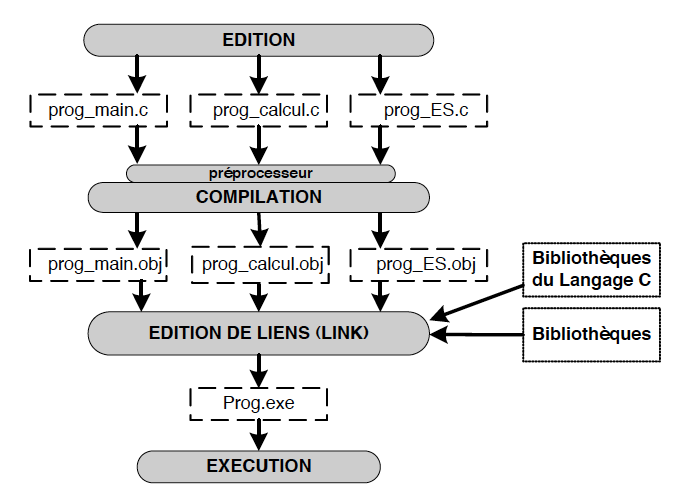
\includegraphics[width=.8\textwidth]{./figures-pdf/compilation}
{\tiny https://public.iutenligne.net/informatique/algorithme-et-programmation/priou/LangageC/}
\end{frame}

%%%%%%%%%%%%%%%%%%%%%%%%%%%
\begin{frame}[plain, fragile]
\frametitle{Fichier d'entête}

\begin{block}{Fichier d'entête}
Les fichiers en‐tête tels que {\tt stdio.h}, {\tt math.h}, etc.  sont des fichiers sources qui contiennent des prototypes des fonction (ex. {\tt printf}), des macro‐instructions (ex. {\tt getchar}), des constantes symboliques (ex. {\tt NULL}, {\tt M\_PI})... Ces fichiers sont utilisés par le préprocesseur pour compléter les fichiers sources : le préprocesseur remplace littéralement la directive {\tt \#include <fic.h}> par le texte contenu dans le fichier {\tt fic.h}.
\end{block}

\begin{block}{Inclusions multiples}
Pour éviter qu'un fichier d'entête soit inclus plusieurs fois, on utilise une macro de protection :
\begin{lstlisting}[language=C]
	#ifndef FOO_H
	#define FOO_H
		... contenu de foo.h
	#endif /* !FOO_H */
\end{lstlisting}

On peut aussi utiliser la directive de préprocesseur {\tt \#pragma once}, mais elle n'est pas forcément prise en charge par tous les compilateurs.

\end{block}


\end{frame}


%%%%%%%%%%%%%%%%%%%%%%%%%%%
\begin{frame}[plain]
\frametitle{La bibliothèque standard}
\begin{quote}
La bibliothèque standard du C est une collection maintenant normalisée d'en-têtes et de routines utilisées pour implémenter des opérations courantes, telles que les entrées/sorties et la gestion des chaînes de caractères, dans le langage C. [\href{https://fr.wikipedia.org/wiki/Bibliothèque_standard_du_C}{wikipedia}]
\end{quote}

Quelques librairies que nous allons utiliser :
\begin{itemize}
	\item {\tt <stdio.h>} : Fournit les capacités centrales d'entrée/sortie du langage C, comme la fonction {\tt printf}.
	\item {\tt <assert.h>} : Contient la macro {\tt assert}, utilisée pour aider à détecter des incohérences de données et d'autres types de bogues dans les versions de débogage d'un programme.
	\item {\tt <time.h>} : Pour convertir entre différents formats de date et d'heure.
\end{itemize}

\end{frame}

%%%%%%%%%%%%%%%%%%%%%%%%%%%
\begin{frame}[plain, fragile]
\frametitle{Focus sur la fonction {\tt printf}}
Prototype :
\begin{lstlisting}[language=C]
	int printf(const char* format, ...);
\end{lstlisting}

Une instruction de formatage peut-être utilisé ainsi avec le format précédé de \%, qui sera associé au nom de la variable qu'on veut afficher.


Quelques librairies que nous allons utiliser :
\begin{table}[htdp]
\begin{center}
\begin{tabular}{|l|c|}
\hline
\bf Type	& \bf Lettre\\
\hline
int	&\%d\\
long	&\%ld\\
short	 & \%hd\\
float/double &	\%f\\
char	& \%c\\
string (char*)	& \%s\\
pointeur (void*)	& \%p\\
entier hexadécimal	& \%x\\
entier octal	& \%o\\
entier non signé &\%u\\
\hline
\end{tabular}
\end{center}
\label{default}
\end{table}%

Exemple :
\begin{lstlisting}[language=C]
	long nombre1 = 400, nombre2 = 500;
	printf("Le nombre 1 est egal a %ld et le nombre 2 a %ld", nombre1, nombre2);
\end{lstlisting}

\end{frame}

%%%%%%%%%%%%%%%%%%%%%%%%%%%
\begin{frame}[plain]
\frametitle{Gestion de la mémoire}

 Le langage C propose trois méthodes principales pour allouer de la mémoire aux objets :
\begin{enumerate}
\item {\bf Allocation statique} : l'espace pour l'objet est alloué dans le binaire au moment de la compilation ; ces objets ont une durée de vie tant que le binaire qui les contient est chargé en mémoire.
\item {\bf Allocation automatique} : des objets temporaires peuvent être stockés sur {\bf la pile}  ({\it stack}), et cet espace est automatiquement libéré et réutilisable après la sortie du bloc dans lequel ils sont déclarés.
\item {\bf Allocation dynamique} : des blocs de mémoire de taille arbitraire peuvent être attribués dans une région de la mémoire appelée {\bf le tas} ({\it heap}) pendant l'exécution à l'aide de fonctions de la bibliothèque standard ({\tt stdlib.h}) ; ces blocs persistent jusqu'à ce qu'ils soient libérés ultérieurement pour pouvoir être réutilisés.
\end{enumerate}


\end{frame}
%%%%%%%%%%%%%%%%%%%%%%%%%%%
\begin{frame}[plain, fragile]
\frametitle{Allocation dynamique}

\begin{block}{Malloc : {\tt void *malloc(size\_t size)}}
Alloue {\tt size} d'octets et renvoie un pointeur sur la mémoire allouée.  La mémoire n'est pas initialisée.
\begin{lstlisting}[language=C]
	double * v = (double *)malloc(12*sizeof(double)); // reservation d'un espace memoire de 12 doubles
\end{lstlisting}
\end{block}

\begin{block}{Free : {\tt void free(void *ptr)}}
Libère l'espace mémoire pointé par un {\tt ptr}, qui doit avoir été retourné par un appel précédent à malloc() ou à des fonctions apparentées. ou d'une fonction apparentée. 
\begin{lstlisting}[language=C]
	free(v);
\end{lstlisting}
\end{block}

\begin{block}{Calloc : {\tt void *calloc(size\_t nitems, size\_t size)}}
Alloue de la mémoire pour un tableau de {\tt nitems} d'un octet chacun et renvoie un pointeur sur la mémoire allouée. La mémoire est mise à zéro. Renvoie un pointeur unique qui peut être passé à free().
\begin{lstlisting}[language=C]
	int *a =  (int *)calloc(12, sizeof(int)); // allocation et mise a zero de 12 entiers de type int
\end{lstlisting}
\end{block}


\end{frame}

%%%%%%%%%%%%%%%%%%%%%%%%%%
\begin{frame}[plain]
\frametitle{Un peu de pratique avec le TD0}

\begin{block}{Objectifs}
\begin{itemize}
	\item Installer les outils (voir \href{https://gitlab.univ-nantes.fr/hladik-pe-1/ecn-gpu-cours/-/blob/main/HowTo/Hwt1-remote/GPGPU_Hwt_remote.pdf}{guide d'installation})
	\item Compiler avec {\tt gcc} et exécuter un code
	\item Coder un petit programme en C
\end{itemize}
\end{block}
\end{frame}
%%%%%%%%%%%%%%%%%%%%%%%%%%



\end{document}